% pre-amble section
\documentclass[11pt,english]{article}
\usepackage[utf8]{inputenc}
\usepackage{geometry}
\usepackage{babel}
\usepackage{hyperref}
\usepackage{graphicx}
\usepackage{appendix}
\usepackage{listings}
\usepackage{caption}
\usepackage{xcolor}

\geometry{legalpaper, margin=1.25in}

\lstdefinestyle{DOS}
{
    backgroundcolor=\color{black},
    basicstyle=\scriptsize\color{white}\ttfamily
}

\title{Herbert\\Autonomous Robotic Rubik's Cube Solver}
\author{
    Jonathan Whitaker\\
    \textt{jon.whitaker@utah.edu}
    \and
    Dylan Lytle\\
    \textt{dylan.lytle@utah.edu}
    \and
    Matt Frandsen\\
    \textt{matt.frandsen@utah.edu}
    \and
    Li Lao\\
    \textt{li.lao@utah.edu}
}
\date{April 2015}
% end of pre-amble

% document content
\begin{document}

\maketitle

\tableofcontents

\section{Abstract}
Project Herbert is an autonomous robotic Rubik's Cube solver that is composed of a complex network of mechanical and electrical devices. In this project our team will be interfacing with these complex mechanical and electrical devices so as to design and create an autonomous robot that is capable of achieving record-breaking Rubik's Cube solution sequences.  This project will be an integration of various technologies including: mechanical actuators, electrical stepper motors, single-board computers, field-programmable gate arrays (FPGAs), and video cameras.

\section{Introduction}
The purpose of this project is to create an autonomous robotic Rubik's Cube solver through the integration of several components. The main components needed in our project include video cameras, electrical stepper motors, mechanical actuators, a single-board computer (SBC), and an FPGA. The video cameras connect to the computer through standard USB 2.0 protocol \cite{USB 2.0}. The video cameras are responsible for capturing the initial configuration of the Rubik's Cube, and the single board computer is responsible for processing the video frame information and generating a matrix model for the initial state of the cube. After generating a matrix model for the initial cube, the computer will then apply Kociemba's algorithm \cite{Kociemba} (an optimal algorithm used to solve a Rubik's Cube) to generate a solution sequence that can be processed sequentially. The solution sequence that Kociemba's algorithm will return will be in the standard notation used in Rubik's Cube discussion and theory (see Appendix \ref{sec:Appendix A}). As each solution sequence is processed, the computer will communicate through an RS232 serial connection to an FPGA board which will drive the mechanical actuation and stepper motor rotations needed to physically manipulate the cube. The FPGA will act as a system control board and will be responsible for controlling the actions of two motor control boards and a relay board used to trigger the mechanical actuators. An overview of this process can be found below in Fig. \ref{fig:System Block Diagram} of section \ref{sec:Project Design}.

Upon completion of the robotic Rubik's Cube solver, if time permits, we hope to take Project Herbert one step further and obtain a Guinness World Record for the fastest robot to solve a Rubik's Cube. CubeStormer3 is the current record holder \cite{GuinnessWR}. The uniqueness of this project is rooted in the optimizations that we will have to make in each component of our system, especially the electro-mechanical stepper motors and the mechanical actuators. We will have to fine-tune these mechanical components to perform physical operations quicker than the human eye in order to obtain record-breaking speed. In this process we will have to maintain the precision needed to rotate the cube.

\section{Project Design}
\label{sec:Project Design}

\begin{figure}[!ht]
\centering
\includegraphics{"Herbert System Diagram".pdf}
\caption{Herbert Block Diagram}
\label{fig:System Block Diagram}
\end{figure}

\subsection{Capturing the Cube with OpenCV}
\label{sec:opencv}

\subsubsection{Camera Orientation}
As seen in Fig. \ref{fig:System Block Diagram}, two cameras will be connected to a SBC through a standard USB 2.0 connection. Each one of these cameras is responsible for capturing exactly three of the six faces of the cube. One camera will capture the front, top, and left faces of the cube. The other camera will be responsible for capturing the back, bottom, and right faces of the cube. To do this, each camera will be positioned so that it faces the corner piece that connects the edges of the faces it is responsible for capturing. An example of this cube orientation is shown in Fig. \ref{fig:Camera Positioning}.

\begin{figure}[!ht]
\centering
\includegraphics[scale=0.25]{"Rubik's Cube Positioning".png}
\caption{Camera Positioning}
\label{fig:Camera Positioning}
\end{figure}

\subsubsection{Utilizing OpenCV for Image Processing}
\label{sec:image processing}
OpenCV is an open source computer vision and machine learning software library \cite{OpenCV}. We will be leveraging this library to perform image analysis on a Rubik's Cube, which will allow us to generate a matrix model for any cube orientation. The OpenCV library will be installed on the SBC, which will enable us to capture and analyze video frames from the USB connected cameras.

Capturing the faces of a cube requires three primary operations:

\begin{enumerate}
  \item \textbf{Grayscale conversion} -
 A video frame will be captured and converted to Grayscale using OpenCV's \textit{cvtColor} function \cite{cvtColor}. Grayscale conversion transforms RGB pixel values into black and white intensity values \cite{Grayscale}. Converting to Grayscale allows an easy transformation to a binary (black and white) image, which is used to filter out features that are not important.
  \item  \textbf{Canny edge detection} -
 Canny edge detection is a multi-stage algorithm used to detect a wide range of edges in an image \cite{Canny Edge Detection}. We will be using OpenCV's \textit{Canny} function \cite{OpenCV Canny} to identify the edges of the Rubik's Cube, which, when combined with contour filtering, will allow us to dynamically identify the planes in the frame that represent the three faces of the cube.

  \item \textbf{Contour filtering} -
 Contour filtering will be used to identify the contours of the Rubik's Cube within the image. OpenCV's \textit{findContours} function \cite{findContours} will allow us to identify the region of space in the image where the Rubik's Cube resides. Likewise, it will enable us to identify individual cubelets on each of the three faces of the cube.
\end{enumerate}

After the individual cubelets have been identified within the image, a matrix model like that shown in Fig. \ref{fig:matrix layout} will be generated. Each individual position (U1, U2, F1, F2, etc.) can be represented as a single ASCII character indicating the color at that cubelet position. Table \ref{table:cubelet representation} defines the mapping scheme we will employ for the Rubik's Cube matrix model. Once this matrix model has been generated for the cube, we will pass it on to an application known as \textit{Kcube}. Kcube will process the cube permutation (see \ref{sec:Kcube}), apply Kociemba's algorithm, and generate a solution sequence.

\begin{figure}[!ht]
\centering
\begin{verbatim}
             |************|
             |*U1**U2**U3*|
             |************|
             |*U4**U5**U6*|
             |************|
             |*U7**U8**U9*|
             |************|
|************|************|************|************|
|*L1**L2**L3*|*F1**F2**F3*|*R1**R2**F3*|*B1**B2**B3*|
|************|************|************|************|
|*L4**L5**L6*|*F4**F5**F6*|*R4**R5**R6*|*B4**B5**B6*|
|************|************|************|************|
|*L7**L8**L9*|*F7**F8**F9*|*R7**R8**R9*|*B7**B8**B9*|
|************|************|************|************|
             |************|
             |*D1**D2**D3*|
             |************|
             |*D4**D5**D6*|
             |************|
             |*D7**D8**D9*|
             |************|
\end{verbatim}
\caption{Rubik's Cube matrix representation}
\label{fig:matrix layout}
\end{figure}

\begin{table}[!ht]
\centering
\begin{tabular}{|c|c|}
\hline
\textbf{COLOR} & \textbf{CHARACTER} \\ \hline
WHITE          & 'W'              \\ \hline
RED            & 'R'              \\ \hline
BLUE           & 'B'              \\ \hline
GREEN          & 'G'              \\ \hline
ORANGE         & 'O'              \\ \hline
YELLOW         & 'Y'              \\ \hline
\end{tabular}
\caption{Cubelet color to ASCII character mapping}
\label{table:cubelet representation}
\end{table}

\subsection{Kcube and the Solution Sequence}
\label{sec:Kcube}
Kcube is a C++ application developed by Greg Schmidt that utilizes Kociemba's two-phase algorithm which uses two stages of an iterative depth first search algorithm \cite{The Two-Phase Algorithm}. The Kcube application will be used to generate the solution sequence needed to solve the Rubik's Cube that was captured during the image processing phase. The matrix model generated from the image processing phase will allow us to provide Kcube's command-line interface with the cube representation needed to generate a solution sequence. Kcube's command-line interface takes six parameters, one for each face of the cube. The values for these parameters are the color characters at each of the cubelet locations for that face (as seen in Fig. \ref{fig:matrix layout}). For example, to solve the scrambled cube shown in Fig. \ref{fig:scrambled cube} you would invoke Kcube with the following command:

\begin{lstlisting}[style=DOS]
Microsoft Windows [Version X.X.XXX]
Copyright (c) 2015 Microsoft Corporation. All rights reserved.

c:>kcube L:GGWWOWBRB F:GWGBGYWBO U:YOOOWYROY D:ORGWYYYRB R:OGBBRYWRR B:YBROBGWGR
\end{lstlisting}

Kcube will then process the input parameters and generate a sequence of twenty-three or less moves (see \ref{sec:fundamental moves}) that, when applied to the cube, will solve the cube. Each move will be mapped to a unique integer value (see Table \ref{table:moves table}), and these values will be transmitted sequentially over an RS232 serial connection to the FPGA control board, at which point the control board will take responsibility for controlling the electro-mechanical stepper motors and mechanical actuators needed to physically manipulate the cube.


\begin{figure}[!ht]
\centering
\includegraphics[scale=1.25]{"Scrambled Cube".jpg}
\caption[]{}
\label{fig:scrambled cube}
\end{figure}

\begin{table}[!ht]
\centering
\begin{tabular}{|c|c|c|c|c|c|}
\hline
\textbf{MOVE} & \textbf{VALUE} & \textbf{MOVE} & \textbf{VALUE} & \textbf{MOVE} & \textbf{VALUE} \\ \hline
F             & 1              & R             & 7              & D             & 13             \\ \hline
F'            & 2              & R'            & 8              & D'            & 14             \\ \hline
F2            & 3              & R2            & 9              & D2            & 15             \\ \hline
L             & 4              & U             & 10             & B             & 16             \\ \hline
L'            & 5              & U'            & 11             & B'            & 17             \\ \hline
L2            & 6              & U2            & 12             & B2            & 18             \\ \hline
\end{tabular}
\caption{Cube moves to integer mapping}
\label{table:moves table}
\end{table}


\subsection{Electro-mechanical Stepper Motors}
\label{sec:Stepper Motors}

\subsection{Mechanical Actuators}
\label{sec:Mechanical Actuators}
In order to achieve a six arm design, each arm must actuate in and out to make
room for the other arms. This actuation process is a time critical component of
the design, and therefore needs to be as fast as possible.  Initially the
implementation of the arm actuation was using motors.  Testing showed that using
motors to convert rotary motion into linear motion, or using a linear motor
actuator were too slow  and or too expensive to obtain the desired result.
Pneumatic actuation was the solution to this problem.  Each of the arms will
be attach to a double action pneumatic air cylinder as show in
figure \ref{fig:Pneumatic Air Cylinder}.

\begin{figure}[!ht]
\centering
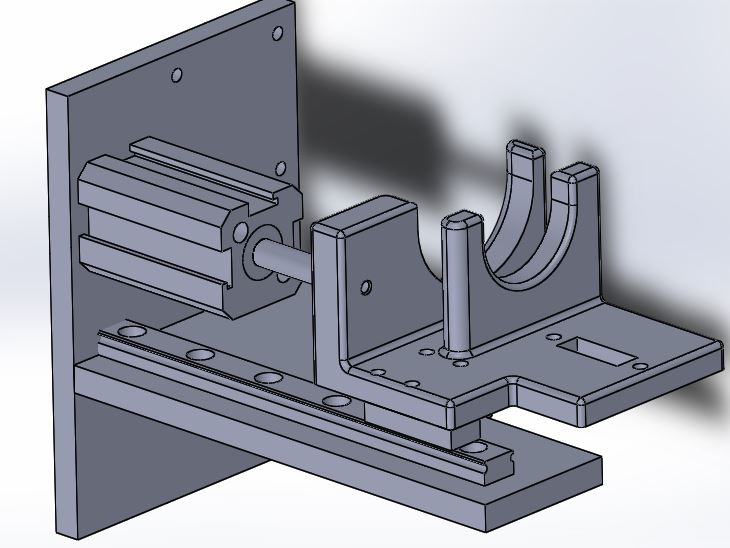
\includegraphics[scale=0.25]{AirCylinder.png}
\caption{Pneumatic Air Cylinder}
\label{fig:Pneumatic Air Cylinder}
\end{figure}. 

The actuation distance is fixed, and the speed of each actuation is very fast.
Using controls from the FPGA, a relay switch controls coaxial pairs of air
cylinders.  As the relay switches coaxial pairs of arms will either be in the
extended or retracted position. Potential algorithm optimizations and more
stable cube manipulations  are obtained by simultaneously extending and
retracting coaxial arms.The linear actuation motion gives the ability for the
arms to extend encasing two sides of the cube in the sockets of the arms, after
which the stepper motor will spin the arm performing the given move of the
solution for the cube. Each air cylinder will be provided approximately
80-100 psi supplied from an air compressor or air tank. To protect against any
collisions, and damages to our project, only one pair of arms will be allowed
to be in the extended position at any given time.


\section{Schedule}
\section{Required Resources}
\section{Summary}
\section{Acknowledgements}
Our team would like to thank BioFire Defense LLC, Point Grey Research Inc., and Futura Industries for all the support and resources they have provided us. Your contributions are greatly appreciated.


\begin{figure}[!htb]
\minipage{0.32\textwidth}
  
\includegraphics[width=\linewidth]{biofire_logo.png}
  \label{fig:biofire_logo}
\endminipage\hfill
\minipage{0.32\textwidth}
  
\includegraphics[width=\linewidth]{point_grey.png}
  \label{fig:point_grey}
\endminipage\hfill
\minipage{0.32\textwidth}%
  
\includegraphics[width=\linewidth]{futura_indust.jpg}
  \label{fig:futura_indst}
\endminipage
\label{fig:project_sponsors}
\end{figure}

BioFire Defense has given us the various control boards and mechanical components needed for this project. They have also given us access to various prototyping tools including high precision 3D printers and laser cutters. A special thanks goes out to BioFire engineers Logan Taylor (Mechanical), Pat Riley (Electrical/Systems), Matt Murdock (Electrical), and David Nielsen (VP of Product Development). These individuals have provided invaluable time and knowledge to our team.

We'd also like to thank Vladimir Tucakov of Point Grey Research. He has provided our team with their Chameleon CMLN-13S2M-CS camera which we will use for precise and fast image acquisition. Vladimir has also discussed our project and ideas with his colleagues at Point Grey, and they have mentioned featuring our project in their newsletter.

We couldn't put all these components together without a nice chassis to house them all. For this, we would like to thank Futura Industries. They have helped us in the design and construction of the aluminum frame we will use to build Herbert. Another special thanks goes out to Futura's Kenton Frandsen (Mechanical/Manufacturing Engineer) who has assisted in the mechanical design of the arm and frame of our project.

\begin{thebibliography}{9}
\bibliographystyle{IEEEtran}

\bibitem{USB 2.0}
\emph{USB 2.0 Specification}
[Online]. Available: \url{http://www.usb.org/developers/docs/usb20_docs/}

\bibitem{Kociemba}
Herbert Kociemba.
\emph{The Two-Phase Algorithm}
[Online]. Available: \url{http://kociemba.org/cube.htm}

\bibitem{GuinnessWR}
Guinness World Records.
\emph{Fastest robot to solve a Rubik's Cube}
[Online]. Available: \url{http://www.guinnessworldrecords.com/world-records/fastest-robot-to-solve-a-rubiks-cub}

\bibitem{OpenCV}
OpenCV Developers Team.
\emph{About OpenCV}
[Online]. Available: \url{http://opencv.org/about.html}

\bibitem{cvtColor}
OpenCV Developers Team.
\emph{Miscellaneous Image Transformations}
[Online]. Available: \url{http://docs.opencv.org/modules/imgproc/doc/miscellaneous_transformations.html#cvtcolor}

\bibitem{Grayscale}
Wikipedia contributors.
\emph{Grayscale}
[Online]. Available: \url{http://en.wikipedia.org/w/index.php?title=Grayscale&oldid=652694198}

\bibitem{Canny Edge Detection}
Wikipedia contributors.
\emph{Canny edge detector}
[Online]. Available: \url{http://en.wikipedia.org/w/index.php?title=Canny_edge_detector&oldid=655662708}

\bibitem{OpenCV Canny}
OpenCV Developers Team.
\emph{Feature Detection}
[Online]. Available: \url{http://docs.opencv.org/modules/imgproc/doc/feature_detection.html?highlight=canny#canny}

\bibitem{findContours}
OpenCV Developers Team.
\emph{Structural Analysis and Shape Descriptors}
[Online]. Available: \url{http://docs.opencv.org/modules/imgproc/doc/structural_analysis_and_shape_descriptors.html?highlight=findcontours#findcontours}

\bibitem{Basic Cube Notation}
Joseph Converse.
\emph{Basic Notation}
[Online]. Available: \url{http://astro.berkeley.edu/~converse/rubiks.php?id1=basics&id2=notation}

\bibitem{The Two-Phase Algorithm}
Herbert Kociemba
\emph{The Two-Phase Algorithm}
[Online]. Available: \url{http://kociemba.org/twophase.htm}
\end{thebibliography}

\appendix
\section{Rubik's Cube Notation and Terminology}
\label{sec:Appendix A}
In order to solve a cube, it is standard to define the terminology and orientation layout used in Rubik's Cube theory and analysis. This section describes the basic notation that is used throughout this document.

\subsection{Faces}
A Rubik's Cube is composed of six faces: right (\textbf{R}), left (\textbf{L}), up (\textbf{U}), down (\textbf{D}), front (\textbf{F}), and back (\textbf{B}) (see Fig. \ref{fig:Cube Orientation}). The exact color of each face is relative to the orientation in which you are holding the cube. For example, if you align the blue face towards you then the blue face is defined as the front face. Each face can be rotated in two different directions: \textit{clockwise} or \textit{counter-clockwise}. These rotations are defined as the direction of rotation when looking directly at that face.

\begin{figure}[!ht]
\centering
\includegraphics{"Cube Orientation".png}
\caption{Cube orientation}
\label{fig:Cube Orientation}
\end{figure}

\subsection{Fundamental Moves}
\label{sec:fundamental moves}
The most fundamental moves are 90-degree clock-wise rotations for each of the faces outlined above. These moves are outlined below \cite{Basic Cube Notation}:

\begin{itemize}

\item{\textbf{R}} - Indicates a 90-degree clockwise rotation of the right face such that the side on top rotates towards the back.
\item{\textbf{L}} - Indicates a 90-degree clockwise rotation of the left face such that the side on top rotates towards the front.
\item{\textbf{U}} - Indicates a 90-degree clockwise rotation of the upper face such that the side in front moves to the left.
\item{\textbf{D}} - Indicates a 90-degree clockwise rotation of the downward face such that the side in front moves to the right.
\item{\textbf{F}} - Indicates a 90-degree clockwise rotation of the front face such that the side on top moves to the right.
\item{\textbf{B}} - Indicates a 90-degree clockwise rotation of the back face such that the side on top moves to the left.
\end{itemize}

\subsection{Modifiers}
For each of the fundamental moves above, there are modifiers that can be appended to the move to change the rotation of the face. My example below uses \textbf{L} as the base move, but these modifiers can be applied to any of the fundamental moves.

\begin{itemize}
\item \textbf{L'} - Indicates a 90-degree counter-clockwise rotation of the left face such that the side on top rotates towards the back (opposite direction as that defined above).
\item \textbf{L2} - Indicates a 180-degree rotation of the left face (two rotations).
\end{itemize}

\subsection{Cubelets}
A cubelet refers to a particular piece on the cube. Cubelets are categorized based on their position. There are three types of cubelets: center cubelets, edge cubelets, and corner cubelets (see Fig. \ref{fig:cubelet_categories}). A center cubelet is unique. All other cubelets revolve around the center cubelets, they never move (go ahead, try and move the center piece). Edge cubelets connect two face pieces together at an edge. A corner cubelet connects three pieces together at the corner of the cube.

\begin{figure}[!htb]
\minipage{0.32\textwidth}
  \includegraphics[width=\linewidth]{"Center cubelets".png}
  \label{fig:center_cubelets}
\endminipage\hfill
\minipage{0.32\textwidth}
  \includegraphics[width=\linewidth]{"Edge cubelets".png}
  \label{fig:edge_cubelets}
\endminipage\hfill
\minipage{0.32\textwidth}%
  \includegraphics[width=\linewidth]{"Corner cubelets".png}
  \label{fig:corner_cubelets}
\endminipage
\caption{Cubelet categories}
\label{fig:cubelet_categories}
\end{figure}



\end{document}
% end of document content
